\newpage
\genHeader
\fancyfoot[RO]{ $\triangleright$ \hyperlink{projectStructure vis}{Next [visual]\hspace{0.2cm}} \\ $\triangleright$ \hyperlink{projectStructure tex}{Next [textual]}}

\section{Validate your installation with JUnit}

\begin{itemize}

\item[$\blacktriangleright$] In\hypertarget{validate common}{} the Eclipse workspace, choose \texttt{Working Sets} as your top level element in the package explorer
(Fig.~\ref{fig_topLevel}). We work with many working sets, and use them to structure the workspace in Eclipse.

\begin{figure}[htbp]
	\centering
  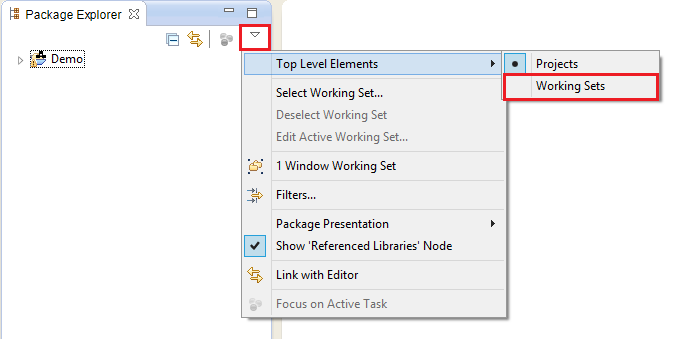
\includegraphics[width=1\textwidth]{eclipse_workingsets}
	\caption{Top Level Elements in Eclipse}
	\label{fig_topLevel}
\end{figure}

\item[$\blacktriangleright$] Locate ``Other Projects/DemoTestSuite.'' This is the testsuite imported with the demo files to make sure everything has been installed and
set up correctly. Right click on the project to bring up the context menu and go to ``Run As/JUnit Test.'' If anything goes wrong, try refreshing by choosing
your metamodel project and pressing  \texttt{F5}, or right-clicking and selecting \texttt{Refresh}.

\vspace{0.5cm}

\begin{figure}[htbp]
	\centering
  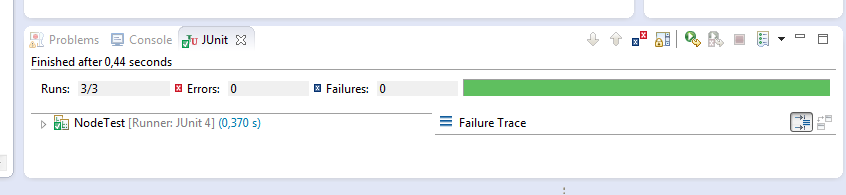
\includegraphics[width=1\textwidth]{eclipse_passedJUnitTest}
	\caption{All's well that ends well\ldots}
	\label{fig_passedTest}
\end{figure}

\vspace{0.5cm}

Congratulations!  If you see a green bar  (Fig.~\ref{fig_passedTest}), then everything has been set up correctly and you are now ready to start metamodelling!

\end{itemize}